% !TeX spellcheck = de_DE
\documentclass[.../Dokumentation.tex]{subfile}
\begin{document}
\section{Fazit}\label{sec-result}
\begin{figure}[H]
\begin{center}
    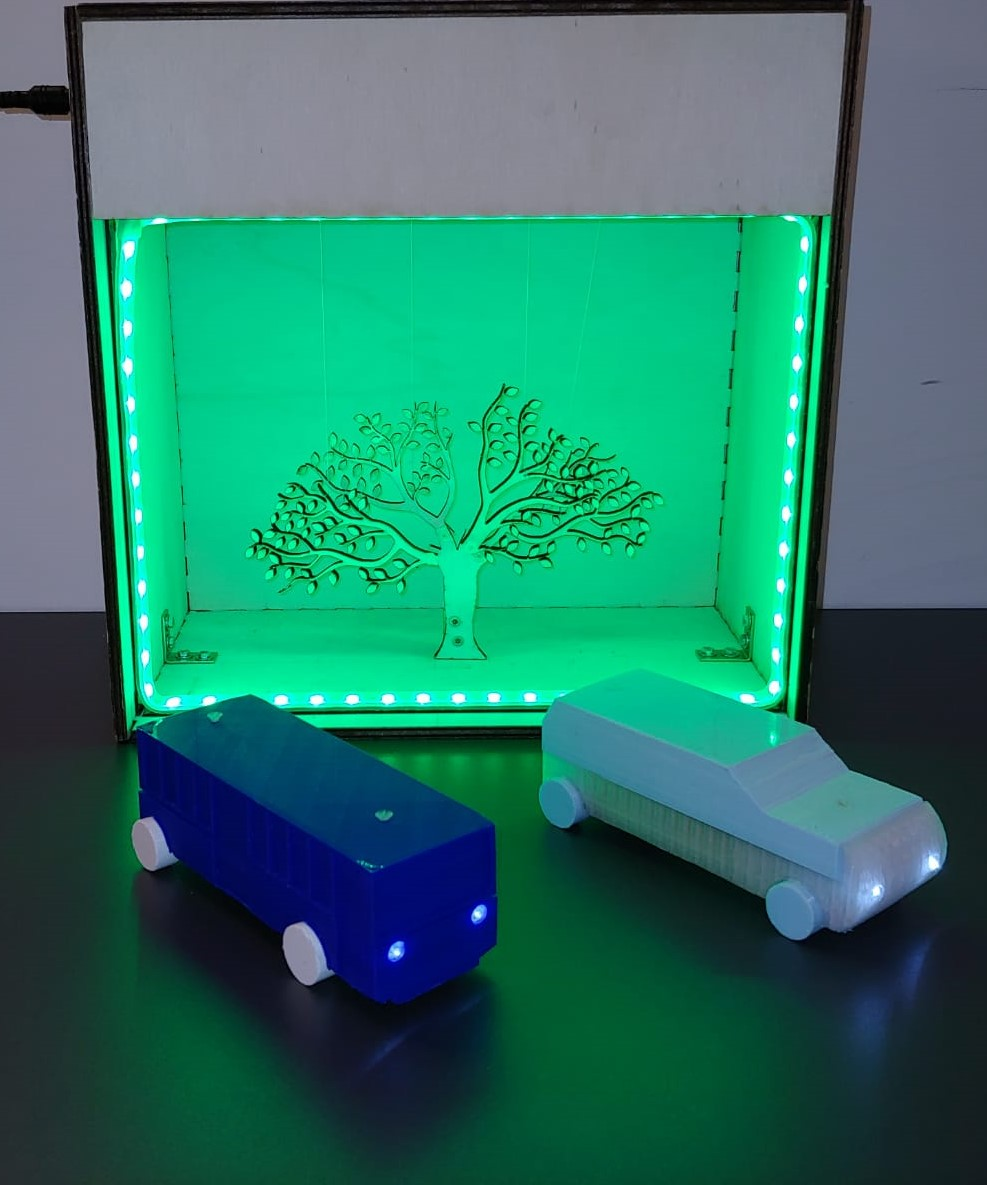
\includegraphics[
        width=0.55\linewidth,
    ]{imgs/final_image.jpeg}
    \caption{Fertiger Prototyp}
    \label{fig-final-prototype}
\end{center}
\end{figure}
\noindent 
Der im Zuge der vier genannten Iterationen entwickelte und geschaffene Prototyp, 
zu sehen in Abbildung \ref{fig-final-prototype},  
wird nachfolgend mit Bezug auf die Projektidee bewertet. Mit den beiden 
Fahrzeugen ist eine anfassbare Schnittstelle zum System realisiert worden. Die 
Fahrzeuge sind mittels 3D-Druck hergestellt und mit je einem Arduino 
ausgestattet. Hierdurch ist die drahtlose Kommunikation mit dem 
dahinterstehenden System möglich. Die Kombination aus der verwendeten Hardware 
und dem Herstellungsprozess der Fahrzeuge ermöglicht es, den gewünschten 
Formfaktor zu erreichen. Trotz der verbauten Hardware sind die Fahrzeuge leicht 
und können auch von Kindern in eine Hand genommen und bedient werden. 
Zur Inbetriebnahme muss lediglich die Stromversorgung der Fahrzeuge mittels 
eines Schalters hergestellt werden. Die Arduinos sind so programmiert und 
konfiguriert, dass sie automatisch die Kommunikation mit dem dahinterliegenden 
System aufnehmen. \\
Dieses System übernimmt Empfang und Verarbeitung der übermittelten Daten sowie 
die Koordination der Darstellung. 
Obwohl die ursprüngliche Idee der Verwendung 
eines Displays verworfen werden musste, wird eine gleichwertige Darstellung auf 
Basis eines beweglichen Baums erzielt. Auch wenn es so nicht mehr möglich ist, 
genaue Messwerte anzuzeigen, wird der Umwelteinfluss verschiedener 
Fahrzeugtypen deutlich. Dieser Eindruck wurde durch den Kontakt mit 
projektfremden Personen, unter anderem im \emph{FabLab}, bestätigt. Wie zuvor 
bei den Fahrzeugen auch muss für den Betrieb lediglich der Raspberry Pi mit 
Strom versorgt werden.\\
Abschließend lässt sich festhalten, dass die zu Beginn formulierte Idee trotz 
angefallener Änderungen erfolgreich umgesetzt werden konnte. Die Komponenten 
des Gesamtsystems interagieren reibungslos miteinander und können den 
gewünschten Lerneffekt bieten, beziehungsweise damit zu einer 
Verhaltensänderung anregen.
\end{document}